\documentclass[cheatsheet.tex]{subfiles}
\begin{document}
Machine learning is the design and analysis of algorithms that improve their performance at some task with experience. The learning may take place offline(face detection), online(adaptive interface) or both(speech recognition). When a machine improves its performance at a given task over time, without reprogramming, it can be said to have learned something. 
\\
\textbf{big picture} We wish to develop methods and tools for building learning machines that can solve problems in combination with available data sets of training examples. 
\\
\textbf{ml problem} Learning involves improving performance at some task T, with experience E, evaluated in terms of performance measure P. 
\\
\textbf{learning problem Components} Task: the behavior or task that's being improved. Data: the experiences that are being used to improve performance in the task. Measure of performance: Provide more accurate solutions, cover a wider range of problems, Obtain answers more economically, Simplify codified knowledge, New skills that were not presented initially.
\\
\textbf{Machine learning ingredients} Prior assumptions, Data, Representation, Model / hypothesis space. Feedback / learning signal, Learning algorithm, Evaluation.
\\
\textbf{Key types} Supervised, Semi-supervised, Unsupervised(find structure in the data), Reinforcement(occasional, delayed information)
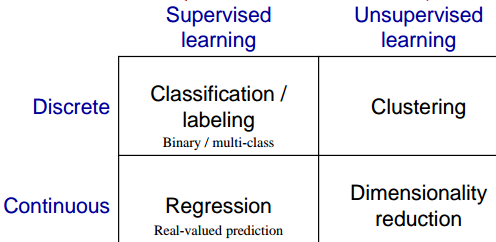
\includegraphics[width=.6\linewidth]{problems.png}\\
\textbf{dataset} \textbullet Training data is used for learning the parameters of the models, \textbullet Validation data is used to decide which model to employ, Sometimes reduced to training and testing a single mode (no validation step) \textbullet Test data is used to get a final, unbiased estimate of how well the model works. 
\\
\textbf{AI vs ML} Deductive reasoning vs Inductive reasoning. \textbullet Learning from a set of known facts and rules to produce additional rules or conclusions that are guaranteed to be true. \textbullet Learning from a set of examples to produce a general rules. The rules should be applicable to new examples, but there is no guarantee that the result will be correct.
\\
\textbf{Homogeneous coordinates} embeds an N-dimensional representation in an N+1-dimensional space Advantage: The decision boundary passes through the origin of the extended coordinate system
\\
\textbf{Overfitting} Learning that results in good performance on the training data but poor performance on the real task
\\
\textbf{Generalization} generalize to the range of inputs/data that will be seen - not just solutions that work well on the training data. model the true regularities in the data and to ignore the noise in the data
\\
\textbf{Reducing model complexity} Ockham's Razor, Prefer the simplest hypothesis that is consistent with the data
\\
\textbf{dimentionality} Distance measures lose their usefulness in high dimensionality. intrinsic dimensionality is lower and the problem is feasible if the relevant dimensions can be identified. 
\\
\subsection{tasks}
A task requires an appropriate mapping -- a model -- from data described by features to outputs. Obtaining such a model from training data is what constitutes a learning problem. Tasks are addressed by models. Learning problems are solved by learning algorithms that produce
models.
\\
\textbf{tasks}, an abstract representation of the problem we want to solve.\textbullet Classification -- assign the target variable to one of N states. \textbullet Regression -- assign the target variable to a real-valued (scalar or vector) function of the input. \textbullet Clustering -- grouping data without prior information. \textbullet Association rule learning \textbullet Subgroup discovery \textbullet Anomaly detection 
\\
\textbf{predictive and descriptive} \textbullet predict/estimate a target variable from features \textbullet  exploiting underlying structure in the data, finding patterns. 
\subsection{models}
a mapping from data points to outputs.
\\
\textbf{Geometric models} use intuitions from geometry such as separating
(hyper)planes, linear transformations and distance metrics. \textbf{Probabilistic models} view learning as a process of reducing uncertainty, modelled by means of probability distributions
\textbf{Logical models} are defined in terms of easily interpretable logical expressions
\\
\textbf{Grouping models} divide the instance space into segments; in each segment a very simple (e.g., constant) model is learned(Don't distinguish between individual instances within each segment, a finite (possibly coarse) resolution of the instance space)\\ 
\textbf{Grading models} learning a single, global model over the instance space.(Infinite resolution (in theory) possible, can distinguish between arbitrary instances)
\\
\textbf{probabilistic models} aim to model the relationship between the feature values X and the target variables Y using probability distributions. Predict Y based on X and the posterior distribution P(Y | X) using Bayes'Rule. 
\\
\textbf{MAP estimation} or maximum a posteriori (MAP) rule, Choose Y that maximizes the value of P(Y | X). 
\\
\textbf{maximum likelihood estimation} or maximum likelihood (ML) rule, Choose Y that maximizes the value of P(X | Y).
\\
\textbf{generative model} a probabilistic model from which we can sample values of all the data variables(Alternative: discriminative models) 
\\
\textbf{Logical models} focus at the level of human reasoning. often provide explanations for their results. often organized in tree structures: feature trees -- that iteratively partition the space of all possible inputs (the instance space). Feature trees whose leaves are labelled with classes are called \textbf{decision trees}
\subsection{features}
Features -- how we describe our data objects. Features are measurements performed on instances.  
\\
\textbf{feature construction} transform the features into a new feature space, to make the
measurements in the appropriate coordinate system. Encapsulate the key similarities and differences in the data, Are robust to irrelevant parameters and transformations, Have a high signal-to-noise ratio. 
\\
\textbf{kernel trick} is a way of mapping features into another (often higher dimensional) space to make
the data linearly separable, without having to compute the mapping explicitly.
\\
\textbf{dimensionality reduction} There may be redundancies -- correlations among features, Some of these features may be useless. 
\\
\textbf{intrinsic dimensionality} of (N-dimensional) data describes the real structure of the data embedded in N-space. 
\end{document}
